% $Id: genetics_article.tex,v 1.11 2003/05/29 02:27:31 warnesgr Exp $
%

\documentclass{report}
\usepackage{Rnews}
\usepackage{graphicx}
\setlength{\textheight}{225mm}  % To fit on US-Letter paper
\begin{document}

\author{by Gregory R. Warnes}
\title{The genetics package}
\subtitle{Utilities for handling genetic data}

\maketitle

\section{Introduction}

In my work as a statistician in the Non-Clinical Statistics and
Biostatistical Applications group within Pfizer Global Research and
Development I have the opportunity to perform statistical analysis in
a wide variety of domains.  One of these domains is pharmacogenomics, in
which we attempt to determine the relationship between the genetic
variability of individual patients and disease status, disease
progression, treatment efficacy, or treatment side effect profile.

Our normal approach to pharmacogenomics is to start with a small set
of candidate genes.  We then look for markers of genetic variability
within these genes.  The most common marker types we encounter are
Single Nucleotide Polymorphisms (SNPs).  SNPs are locations where some
individuals differ from the norm by the substitution one of the 4 DNA
bases, adenine (A), thymine (T), guanine (G), and cytosine (C), by a
one of the other bases.  For example, a single cytosine (C) might be
replaced by a single tyrosine (T) in the sequence `CCT\textbf{C}AGC',
yielding `CCT\textbf{T}AGC'.  We also encounter simple sequence length
polymorphisms (SSLP), which are also known as microsatellite DNA.
SSLP are simple reteating patters of bases where the number of repeats
can vary. E.g., at a particular position, some individuals might have
3 repeats of the pattern `CT', `AC\textbf{CTCTCT}AA', while others
might have 5 repeats, `AC\textbf{CTCTCTCTCT}AA'.

Regardless of the type or location of genetic variation, each
individual has two copies of each chromosome, hence two alleles
(variants), and consequently two data values for each marker.  This
information is often presented together by providing a pair of allele
names.  Sometimes a separator is used (e.g.  `A/T'), sometimes they
are simply concatinated (e.g., `AT').

A further layer of complexity arises from the inability of most
laboratory methods to determine which observed variants comes from
which copy of the chromosome.  (Statistical methods are often
necessary to impute this information when it is needed.)  For this
type of data `A/T', and `T/A' are equivalent.

\section{The genetics package}

The genetics package, available from CRAN, includes classes and
methods for creating, representing, and manipulating genotypes
(unordered allele pairs) and haplotypes (ordered allele pairs).
Genotypes and haplotypes can be annotated with chromosome, locus
(location on a chromosome), gene, and marker information.  Utility
functions compute genotype and allele frequencies, flag homozygotes or
heterozygotes, flag carriers of certain alleles, count the number of a
specific allele carried by an individual, extract one or both alleles.
.  These functions make it easy to create and use single-locus genetic
information in \R's statistical modeling functions.

The genetics library also provide a set of functions to estimate and
test for departure from Hardy-Weinberg equilibrium (HWE).  HWE
specifies the expected allele frequencies for a single population when
none of the variant alleles impart a survival benefit.  Departure from
HWE is often indicative of a problem with the laboratory assay, and is
often the first statistical method applied to genetic data.  In
addition, the genetics package provides functions to test for linkage
disequilibrium (LD), the non-random association of marker alleles
which can arise from marker proximity or from selection bias.
Further, to assist in sample size calculations when considering sample
sizes needed when investigating potential markers, we provide a
function which computes the probability of observing all alleles with
a given true frequency.

My primary motivation in creating the genetics library was to overcome
the difficulty in representing and manipulating genotype in
general-purpose statistical packages.  Without an explicit genotype
variable type, handling genetic variables requires considerable string
manipulation, which can be quite messy and tedious.  The
\code{genotype} function has been designed to remove the need to
perform string manupulation by allowing allele pairs to be specified
in any of four commonly occuring notations:

\begin{itemize} 
\item A single vector with a character separator:
  {\small
\begin{verbatim} 
  g1 <- genotype( c('A/A','A/C','C/C','C/A',
                     NA,'A/A','A/C','A/C') )
  g3 <- genotype( c('A A','A C','C C','C A',
                    '','A A','A C','A C'), 
                  sep=' ', remove.spaces=F)
\end{verbatim}
}  


\item A single vector with a positional separator
  {\small
\begin{verbatim}
  g2 <- genotype( c('AA','AC','CC','CA','',
                    'AA','AC','AC'), sep=1 )
\end{verbatim}
}  


\item Two separate vectors
  {\small
\begin{verbatim}
  g4 <- genotype( 
          c('A','A','C','C','','A','A','A'),
          c('A','C','C','A','','A','C','C')
          )
\end{verbatim}
}  

\item A dataframe or matrix with two columns
  {\small
\begin{verbatim}
  gm <- cbind( 
          c('A','A','C','C','','A','A','A'),
          c('A','C','C','A','','A','C','C') ) 
  g5 <- genotype( gm )
\end{verbatim}
}  
\end{itemize}

For simplicity, the functions makeGenotype and makeHaplotype can be
used to convert all of the genetic variables contained in a dataframe
in a single pass.  (See the help page for details.)

A second difficulty in using genotypes is the need to represent the
information in different forms at different times.  To simplify the
use of genotype variables, each of the three basic ways of modeling
the effect of the allele combinations is directly supported by the
\code{genetics} package:
\begin{description}
\item[categorical] Each allele combination acts differently.
  
  This situation is handled by entering the \code{genotype} variable without
  modification into a model.  In this case, it will be treated as a
  factor:

{\small
\begin{verbatim}
lm( outcome ~ genotype.var + confounder )
\end{verbatim}
}
  
\item[additive] The effect depends on the number of copies of a
  specific allele (0, 1, or 2).
  
  The function \code{allele.count( gene, allele )} returns the number
  of copies of the specified allele:
  
{\small
\begin{verbatim}
lm( outcome ~ allele.count(genotype.var,'A') 
              + confounder )
\end{verbatim}
}
  
\item[dominant/recessive] The effect depends only on the presence or
  absence of a specific allele.
  
  The function \code{carrier( gene, allele )} returns a boolean flag
  if the specified allele is present:

{\small
\begin{verbatim}
lm( outcome ~ carrier(genotype.var,'A') 
              + confounder )
\end{verbatim}
}

\end{description}

\section{Implementation}

The basic functionality of the \code{genetics} package is provided by
the \code{genotype} class and the \code{haplotype} class, which is a
simple extension of the former.  Friedrich Leisch and I collaborated
on the design of the \code{genotype} class.  We had four goals: First,
we wanted to be able to manipulate both alleles as a single variable.
Second, we needed a clean way of accessing the individual alleles when
this was required.  Third, a genotype variable should be able to be
stored in dataframes as they are currently implemented in R.  Fourth,
the implementation of genotype variables should be space-efficient.

After considering several potential implementations, we chose to
implement the genotype class as an extension to the in-built factor
variable type with additional information stored in attributes.
Genotype objects are stored as factors and have the class list
\code{c("genotype","factor")}.  The names of the factor levels are
constructed as \code{paste(allele1,"/",allele2,sep="")}.  Since most
genotyping methods do not indicate which allele comes from which
member of a chromosome pair, the alleles for each individual are
placed in a consistent order controlled by the \code{reorder}
argument.  In cases when the allele order is informative, the
\code{haplotype} class, which preserves the allele order, should be
used instead.

The set of allele names is stored in the attribute
\code{allele.names}.  A translation table from the factor levels to
the names of each of the two alleles is stored in the attribute
\code{allele.map}.  This map is a two column character matrix with one
row per factor level.  The columns provide the individual alleles for
each factor level.  Accesing the individual alleles, as performed by
the \code{allele} function, is accomplished by simply indexing into
this table,
\begin{verbatim}
allele.x <- attrib(x,"allele.map") 
alleles.x[genotype.var,which]
\end{verbatim}
where \code{which} is \code{1}, \code{2}, or \code{c(1,2)} as
appropriate.

Finally, there is often additional meta-information associated with a
genotype.  The functions \code{locus}, \code{gene}, and \code{marker}
create objects to store information, respectively, about genetic loci,
genes, and markers.  Any of these objects can be included as part of a
genotype object using the \code{locus} argument. The print and summary
functions for genotype objects properly display this information when
it is present.

This implementation of the genotype class met our four design goals
and offered an additional benefit: in most contexts factors behave the
same as the desired default behavior for genotype objects.
Consequently, relatively few additional methods needed to written.
Further, in the absence of the genetics package, the information
stored in genotype objects is still accessible in a reasonable way.

The \code{genotype} class is accompanied by a full complement of
helper methods for standard R operators ( \code{[]}, \code{[<-},
\code{==}, etc. ) and object methods ( \code{summary}, \code{print},
\code{is.genotype}, \code{as.genotype}, etc. ).  Additional functions for manipulating genotypes include: 

\begin{description}
  
\item[allele] Extracts individual alleles.
  matrix.
  
\item[allele.names] Extracts the set of allele names.
  
\item[homozygote] Creates a logical vector indicating whether both
  alleles of each observation are the same.
  
\item[heterozygote] Creates a logical vector indicating whether the
  alleles of each observation differ.
  
\item[carrier] Creates a logical vector indicating whether
  the specified alleles are present.
  
\item[allele.count] Returns the number of copies of the specified
  alleles carried by each observation.
  
\item[getlocus] Extracts locus, gene, or marker information.
  
\item[makeGenotypes] Convert appropriate columns in a dataframe to
  genotypes or haplotypes

\item[write.pop.file] Creates a 'pop' data file, as used by the
  GenePop (\url{http://wbiomed.curtin.edu.au/genepop/}) and LinkDos
  (\url{http://wbiomed.curtin.edu.au/genepop/linkdos.html}) softare
  packages.
     
\item[write.pedigree.file] Creates a 'pedigree' data file, as used by
  the QTDT software package
  (\url{http://www.sph.umich.edu/statgen/abecasis/QTDT/}).
  
\item[write.marker.file] Creates a 'marker' data file, as used by the
  QTDT software package
  (\url{http://www.sph.umich.edu/statgen/abecasis/QTDT/}).
\end{description}

The genetics package provides four functions related to Hardy-Weinberg Equilibrium:
\begin{description}
\item[diseq] Estimate or compute confidence interval for the
  single marker Hardy-Weinberg disequilibrium
\item[HWE.chisq] Performs a Chi-square test for Hardy-Weinberg equilibrium
\item[HWE.exact] Performs a Fisher's exact test of Hardy-Weinberg equilibrium for two-allele markers.
\item[HWE.test] Computes estimates and bootstrap confidence intervals,
  as well as testing for Hardy-Weinberg equilibrium.
\end{description}
as well as three related to linkage disequilibrium (LD):
\begin{description}
\item[LD] Compute pairwise linkage disequilibrium between genetic markers.
\item[LDtable] Generate a graphical table showing the LD estimate,
  number of observations and p-value for each marker combination,
  color coded by significance.
\item[LDplot] Plot linkage disequilibrium as a function of marker location.
\end{description}
and one function for sample size calculation:
\begin{description}
\item[gregorius] Probability of Observing All Alleles with a Given
  Frequency in a Sample of a Specified Size.  
\end{description}
The algorithms used in the HWE and LD functions are beyond the scope
of this article, but details are provided in the help pages or the
corresponding package documentation.

\section{Example}

Here is a partial session using tools from the genotype package to
examine the features of 3 simulated markers and thier relationships
with a continuous outcome:

{\small
\begin{verbatim}
> library(genetics)
[...]
> # Load the data from a CSV file
> data <- read.csv("example_data.csv")
> 
> # Convert genotype columns to genotype variables
> data <- makeGenotypes(data)
> 
> ## Annotate the genes 
> marker(data$a1691g) <-
+   marker(name="A1691G",
+          type="SNP",
+          locus.name="MBP2",
+          chromosome=9, 
+          arm="q", 
+          index.start=35,
+          bp.start=1691,
+          relative.to="intron 1")
[...]
> 
> # Look at some of the data
> data[1:5,]
      PID DELTA.BMI c104t a1691g c2249t
1 1127409      0.62   C/C    G/G    T/T
2  246311      1.31   C/C    A/A    T/T
3  295185      0.15   C/C    G/G    T/T
4   34301      0.72   C/T    A/A    T/T
5   96890      0.37   C/C    A/A    T/T
> 
> # Get allele information for c104t
> summary(data$c104t)

Marker: MBP2:C-104T (9q35:-104) Type: SNP

Allele Frequency:
  Count Proportion
C   137       0.68
T    63       0.32

Genotype Frequency:
    Count Proportion
C/C    59       0.59
C/T    19       0.19
T/T    22       0.22

> 
> 
> # Check Hardy-Weinberg Equilibrium
> HWE.test(data$c104t)

        -----------------------------------
        Test for Hardy-Weinberg-Equilibrium
        -----------------------------------

Call: 
HWE.test.genotype(x = data$c104t)

Raw Disequlibrium for each allele pair (D)

  C    T   
C      0.12
T 0.12     

Scaled Disequlibrium for each allele pair (D')

  C    T   
C      0.56
T 0.56     

Correlation coefficient for each allele pair (r)

  C     T    
C  1.00 -0.56
T -0.56  1.00

Overall Values

     Value
  D   0.12
  D'  0.56
  r  -0.56

Confidence intervals computed via bootstrap 
using 1000 samples

             Observed 95% CI           NA's
  Overall D   0.121   ( 0.073,  0.159) 0   
  Overall D'  0.560   ( 0.373,  0.714) 0   
  Overall r  -0.560   (-0.714, -0.373) 0   
             Contains Zero?
  Overall D  *NO*          
  Overall D' *NO*          
  Overall r  *NO*          

Significance Test:

        Exact Test for Hardy-Weinberg Equilibrium

data:  data$c104t 
N11 = 59, N12 = 19, N22 = 22, N1 = 137, N2
= 63, p-value = 3.463e-08



> 
> # Check Linkage Disequilibrium
> ld <- LD(data)
Warning message: 
Non-genotype variables or genotype variables with 
more or less than two alleles detected. These
 variables will be omitted: PID, DELTA.BMI 
in: LD.data.frame(data) 
> ld # text display

Pairwise LD
-----------
               a1691g c2249t
c104t  D        -0.01  -0.03
c104t  D'        0.05   1.00
c104t  Corr.    -0.03  -0.21
c104t  X^2       0.16   8.51
c104t  P-value   0.69 0.0035
c104t  n          100    100
                            
a1691g D               -0.01
a1691g D'               0.31
a1691g Corr.           -0.08
a1691g X^2              1.30
a1691g P-value          0.25
a1691g n                 100
                            

> 
> LDtable(ld) # graphical display
\end{verbatim}

\begin{center}
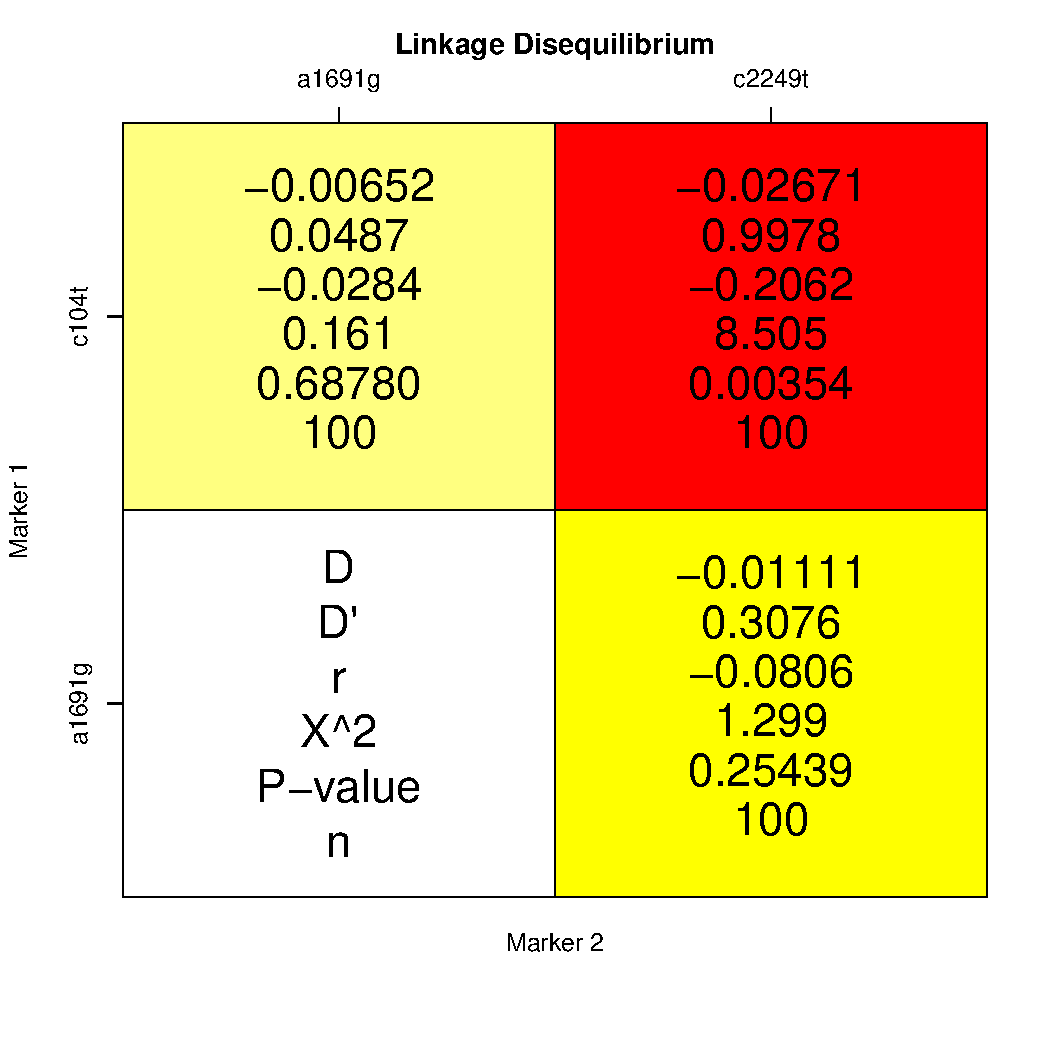
\includegraphics[width=0.5\textwidth]{LD.pdf}
\end{center}
\begin{verbatim}

> # fit a model
> summary(lm( DELTA.BMI ~ 
+                 homozygote(c104t,'C') +
+                 allele.count(a1691g, 'G') +
+                 c2249t, data=data))

Call:
lm(formula = DELTA.BMI ~ homozygote(c104t, "C") + 
    allele.count(a1691g, "G") + c2249t, 
    data = data)

Residuals:
    Min      1Q  Median      3Q     Max 
-2.9818 -0.5917 -0.0303  0.6666  2.7101 

Coefficients:
                           Estimate Std. Error
(Intercept)                 -0.1807     0.5996
homozygote(c104t, "C")TRUE   1.0203     0.2290
allele.count(a1691g, "G")   -0.0905     0.1175
c2249tT/C                    0.4291     0.6873
c2249tT/T                    0.3476     0.5848
                           t value Pr(>|t|)    
(Intercept)                  -0.30     0.76    
homozygote(c104t, "C")TRUE    4.46  2.3e-05 ***
allele.count(a1691g, "G")    -0.77     0.44    
c2249tT/C                     0.62     0.53    
c2249tT/T                     0.59     0.55    
---
Signif. codes:  0 `***' 0.001 `**' 0.01 
                `*' 0.05 `.' 0.1 ` ' 1 

Residual standard error: 1.1 on 95 degrees of 
                         freedom
Multiple R-Squared: 0.176,      
Adjusted R-squared: 0.141 
F-statistic: 5.06 on 4 and 95 DF,  
             p-value: 0.000969 

\end{verbatim}
}

\section{Conclusion}

The current release of the \code{genetics} package, 1.0.0, provides a
complete set of classes and methods for handling single-locus genetic
data as well as functions for computing and testing for departure from
Hardy-Weinberg and linkage disequilibrium using a variety of
estimators.

As noted earlier, Friedrich Leisch and I collaborated on the design of
the data structures.  While I was primarily motivated by the desire to
provide a natural way to include single-locus genetic variables in
statistical models, Fritz also wanted to support multiple genetic
changes spread across one or more genes.  As of the current version,
my goal has largely been realized, but more work is necessary to fully
support Fritz's goal.

In the future I intend to add functions to perform haplotype
imputation and generate standard genetics plots.

I would like to thank Freidrich Leisch for his assistance in designing
the genotype data structure, David Duffy for contributing the code for
the \code{gregarious} and {HWE.exact} functions, and Michael Man for error
reports and helpful discussion.  

I welcome comments and contributions.

\address{Gregory R. Warnes \\
        Pfizer Global Research and Development \\
        \emph{gregory\_r\_warnes@groton.pfizer.com} }

\end{multicols}

\end{document}
